\documentclass[11pt, a4paper]{article}
\usepackage[utf8]{inputenc}

% List of Latex packages to use
\usepackage[margin = 1in]{geometry}
\usepackage{amsfonts,amsmath,amssymb,amsthm}
\usepackage{graphicx,subcaption}
\usepackage{booktabs}
\usepackage{lipsum}
\usepackage{hyperref}
%\usepackage{subfig}
\usepackage{multicol}
\hypersetup{
   colorlinks = true,
   citecolor = blue,
   urlcolor = blue,
   linkcolor = red
}


% Custom Commands
\newcommand{\nindep}{\not\!\perp\!\!\!\perp}
\newcommand{\indep}{\perp\!\!\!\perp}

\begin{document}
% titling

\begingroup
\begin{titlepage}
    \begin{flushright}
           
\includegraphics[width=0.1\textwidth]{isi-logo.png}
    \end{flushright}
   \begin{center}
    \vspace*{2.5cm}
       \textbf{\LARGE Analysis of Impact of Covid19 Pandemic on Stock Prices of Large Tech Video Communication Companies}
       
       
\includegraphics[width=0.8\textwidth]{video-conferencing-statistics.jpeg}
 
       \vspace{1.5cm}
 
       \textsc{\Large A report presented as a part of the course\\ Financial Econometrics, Spring 2021}
 
       \vspace{0.8cm}
        
        \large
        \textbf{Rounak Ghosh}, MB1904\\
        \textbf{Nadim Akhtar}, MB1906\\
        \textbf{Subhrajyoty Roy}, MB1911\\
        \textbf{Monitirtha Dey}, MB1921\\
        

        \vspace{1cm}
       \textbf{Programme :} Master of Statistics (M.Stat. Year II)\\
       \textbf{Institution: } Indian Statistical Institute, Kolkata\\
       \textbf{Date: } \today
       
   \end{center}
\end{titlepage}
\endgroup

\section{Introduction}
Forecasts are an important tool for investors to close successful deals. This gives traders the confidence to know in a timely manner when to buy and sell stocks. Forecasting stock prices is important for market participants because sufficiently accurate forecasts can also provide huge financial benefits for policymakers who are analyzing the market's impact on national or international events. Despite the pressuring need for stock price forecasting and numerous statistical, machine learning, deep learning and computation techniques available~\cite{wiki-stock}, various economic and social factors create uncertainty and volatility in those predictions. 

Infectious diseases have always been a threat to mankind, especially those that are little or not known about. The World Health Organization (WHO) describes a pandemic as ``the spread of a new disease worldwide''~\cite{who-pandemic-defn} and while at such times the greatest concern is saving lives, the next first goal is to save the economy and maintain prosperity. During recent times of the ongoing COVID-19 pandemic, it has become apparent that the study of the pandemic is an influential component of the behaviour of the stock market. From 24 to 28 February 2020, stock markets around the world experienced their biggest one-week decline since the 2008 financial crisis~\cite{wiki-stock-crash}, with traders starting to sell stocks out of fear of imminent recession and market liquidity crisis. As a result, the four-way switch was triggered four times in March. The effect of COVID-19 was not only direct, but indirect effects associated with healthcare policies and lockdown strategies~\cite{guru2021covid}, miscommunication and spread of fake news~\cite{salisu2020predicting} were also some of the social factors that cause the stock market crash in 2020.

When the Coronavirus pandemic began to hit the world, both the academic and corporate industries adopted a study-from-home and work-from-home culture. Consequently, the flexible e-learning tools, video conferencing applications relying on the Internet have proven to be the key to teacher-student interactions~\cite{chen2020impact} in academics, employer-employee relationships in the corporate industry. It has become a very effective solution for everyone involved, keeping the public safe while promoting the useful use of technology, as well as allowing various companies to save budgets of office maintenance costs. In academics, despite various social issues pertaining to internet access inequalities, many agree that continuing online classes proved beneficial by allowing the students to avoid knowledge gaps that could have arisen if students did not have access to education for a long time due to lockdown. Many researchers even suspect that this temporary change to counter the threat of disease spread could become a permanent culture~\cite{bick2020work}, as most of the world has already adapted to the emerging system. 

This radical change in social interactions has significantly boosted the usage of online video conferencing applications over the past year. Among different video conferencing tools, Google Meet, Microsoft Teams, Zoom and Skype are more popular than the rest. Clearly, the associated companies, namely Alphabet Inc (Google) and Microsoft Corporation both have been able to generate enormous revenue by selling their products, which should be reflected in the prices of these particular stocks. Hence, we expect that the intensity of worldwide confirmed covid cases should well be correlated with their stock prices. Therefore, in this project, we aim to examine the effects of the COVID-19 pandemic on the stock prices of Alphabet Inc (Google) and Microsoft Corporation. 

\section{Description of the Data}

The World Health Organization (WHO) declared the outbreak of COVID-19 a Public Health Emergency of International Concern on 30 January 2020~\cite{wiki-covid-syndrome}. So, we restricted our dataset starting from 30th January, 2020 to 30th April, 2021. Among stock prices, our dataset includes daily closing prices of the stocks Alphabet Inc (symbol GOOGL) and Microsoft Corporation (symbol MSFT) collected from Yahoo Finance~\cite{yahoo-finance}. Both of these stocks are registered in the American stock exchange market NASDAQ~\cite{nasdaq}. Figure~\ref{fig:stock-price} shows the line diagram of these two stock prices for the studied timespan. Our dataset also includes the number of daily new confirmed cases of covid on a worldwide basis which are collected from JHU CSSE Github repository~\cite{coviddata}. In addition to these, we believe that the number of google searches about certain keyword terms such as ``google meet", ``microsoft teams", ``skype", ``zoom" and ``covid test", may be useful to quantify the current trend of popularity of video conferencing applications among the masses. Google publishes these aggregated searching data through the Google Trends platform~\cite{google-trends}. 

\begin{figure}
    \centering
    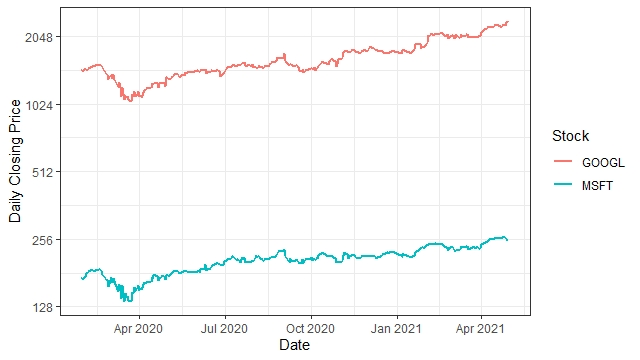
\includegraphics[width = 0.8\textwidth]{figures/plot0.jpeg}
    \caption{Daily closing stock prices for the stocks of Alphabet Inc (GOOGL) and Microsoft Corporation (MSFT)}
    \label{fig:stock-price}
\end{figure}

Google Trends~\cite{google-trends} provides access to a largely unfiltered sample of actual search requests made to Google. It’s anonymized (no one is personally identified), categorized (determining the topic for a search query), and aggregated (grouped together). This allows us to display interest in a particular topic from around the globe or down to city-level geography. Instead of providing the actual number of searches about a particular topic, it normalizes the search data to make comparisons between terms easier. Search results are normalized to the time and location of a query by the following process:

\begin{itemize}
    \item Each data point is divided by the total number of searches in the geography and time range to represent relative popularity. Otherwise, places with the most search volume would always be ranked highest.
    \item The resulting numbers are then scaled on a range of 0 to 100 based on a topic's proportion to all searches on all topics.
    \item Different regions that show the same search interest for a term do not always have the same total search volumes.
    \item Finally, the normalized scores of popularity are rounded to the nearest integer between 0 to 100.
\end{itemize}

We found that Google Trends data containing the whole time range and all the five search terms together have little use since most of the terms have relatively low popularity compared to that of covid related searches, resulting in a normalized score of 0 for most of the time. Hence, we segmented the whole timespan into 4 overlapping segments of 5-6 months, with one month of data common between them. That allowed us to have more descriptive popularity scores, but with different normalization factor for different timespan. For instance, let $x_1, x_2, \dots x_n$ be the original time series. However, for the time span $\{ 1, 2, \dots k, k+1, \dots r \}$, let the observed scores are $y_1, y_2, \dots y_r$ and for the time span $\{ k, k+1, \dots r, r+1, \dots n \}$, let the observed scores are $z_k, z_{k+1}, \dots z_n$. In general, $y_i = x_i / c_1$ and $z_i = x_i / c_2$, where $c_1$ and $c_2$ are possibly different normalization factors to scale the corresponding series in the range 0-100. Since $y_i c_1 = x_i = z_i c_2$ for $i = k, k+1, \dots r$, the ratio $c_1/c_2$ can be approximated by a simple average of the values $z_k/y_k, z_{k+1}/y_{k+1}, \dots z_r/y_r$. This ratio can then be multiplied with the complete $z$-series to obtain a properly scaled version of it which can be easily merged with the $y$-series (Note that after the multiplication, the normalization constant becomes the same as $c_1$). This procedure allowed us to combine the segmented time series of search trends into combined search trends for the whole study period.


\section{Methodologies}\label{sec:methods}

As mentioned earlier, our study focuses on quantifying the effect of worldwide confirmed covid cases on the stock prices of Alphabet Inc (Google) and Microsoft Corporation. It is standard practice in stock price analysis and economics to perform a logarithmic transformation of the prices, which is also done in this case. Figure~\ref{fig:relation1} represents the relationship between the two log-transformed stock prices and daily new confirmed covid cases on a worldwide basis. We observe non-linear relationships between the log-transformed stock prices and daily new confirmed covid cases. To mitigate this, square root transformation and log transformation are two popular options on the covid cases variable. We found that square root transformation performs better for our dataset. This revised variable is then found to have a better linear relationship with the log-transformed stock prices; see Figure~\ref{fig:relation2} for illustration. Therefore, instead of using the number of new confirmed covid cases in our analysis, we use the square root of this variable as an explanatory variable. Also, both the stock prices of Alphabet Inc and Microsoft Corporation should be dependent on the popularity ratings (which are measured by the search indices provided by Google Trends) of their competitors, i.e Skype and Zoom. Naturally, these ratings are also included as explanatory variables.


\begin{figure}[ht]
    \centering
    \begin{subfigure}{0.49\textwidth}
       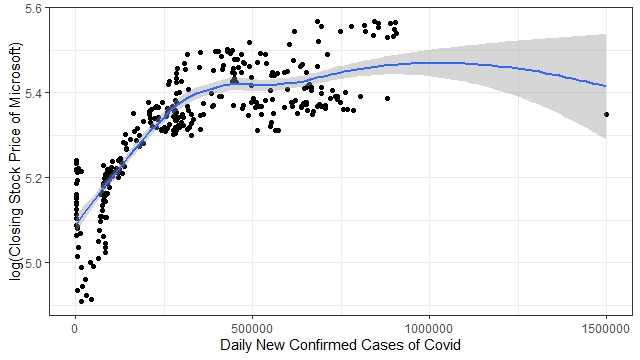
\includegraphics[width = \textwidth]{figures/plot1.jpeg}
    \end{subfigure}
    \begin{subfigure}{0.49\textwidth}
       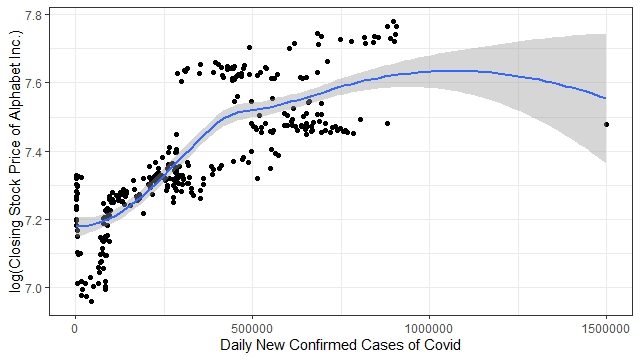
\includegraphics[width = \textwidth]{figures/plot2.jpeg}
    \end{subfigure}
    \caption{Plots of Daily closing stock prices of Alphabet Inc (GOOGL) and Microsoft Corporation (MSFT) vs daily new confirmed covid cases}
    \label{fig:relation1}
\end{figure}



\begin{figure}[ht]
    \centering
    \begin{subfigure}{0.49\textwidth}
       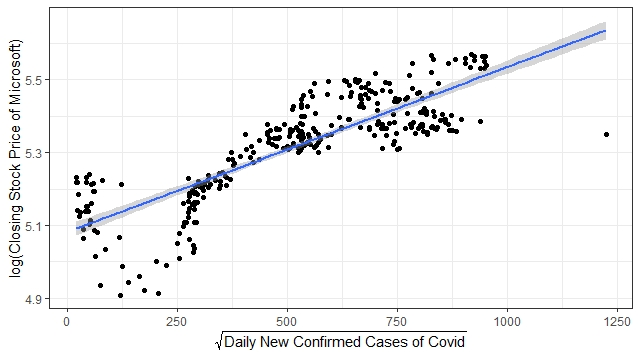
\includegraphics[width = \textwidth]{figures/plot3.jpeg}
    \end{subfigure}
    \begin{subfigure}{0.49\textwidth}
       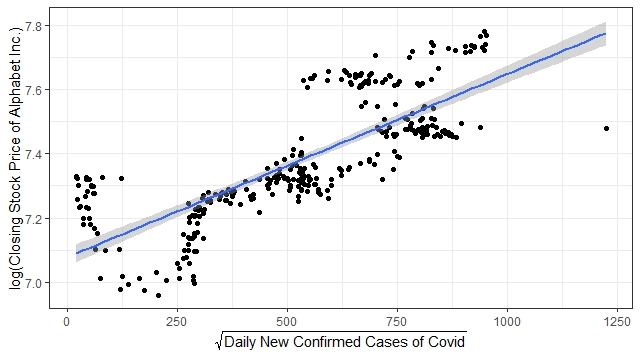
\includegraphics[width = \textwidth]{figures/plot4.jpeg}
    \end{subfigure}
    \caption{Plots of Daily closing stock prices of Alphabet Inc (GOOGL) and Microsoft Corporation (MSFT) vs square root of daily new confirmed covid cases}
    \label{fig:relation2}
\end{figure}

\noindent Let us denote the day-level variables as

\begin{equation}
    \begin{split}
        SP_{G} & = \text{Log-transformed Stock Price of Alphabet Inc (Google)}\\
        SP_{M} & = \text{Log-transformed Stock Price of Microsoft Corporation}\\
        C_{new} & = \sqrt{\text{New confirmed covid cases}}\\
        PR_{G} & = \text{Popularity Rating of Google}\\
        PR_{M} & = \text{Popularity Rating of Microsoft}\\
        PR_{S} & = \text{Popularity Rating of Skype}\\
        PR_{Z} & = \text{Popularity rating of Zoom}
    \end{split}
    \label{eqn:variable-description}
\end{equation}

The popularity ratings are essentially the normalized scores of Google search of a search term as provided by Google Trends~\cite{google-trends}. As discussed above, working with the segmented timespans and merging them allowed the rating to scale proportionately outside the usual range of 0-100, allowing much clear variations in the ratings. Figure~\ref{fig:corr} presents a heat-plot of the Pearson's product moment correlation coefficient between the above variables. Most of the variables turned out to be very much linearly correlated, hence linear regression is a possible choice to model the effect of the variables on the stock prices. The two stock prices are also strongly dependent on each other. This is supported by the scatterplot depicted in Figure~\ref{fig:GvsM}.

\begin{figure}[ht]
    \centering
    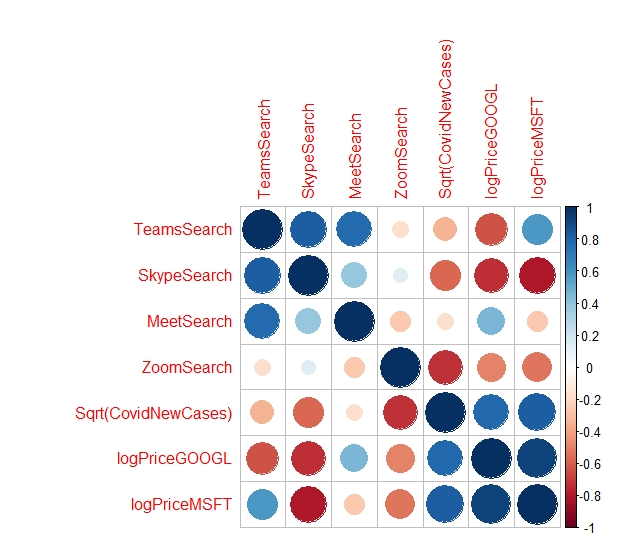
\includegraphics[width = 0.75\textwidth]{figures/plot5.jpeg}
    \caption{Correlations between the seven variables described in Eq.~\eqref{eqn:variable-description}}
    \label{fig:corr}
\end{figure} 

\begin{figure}[ht]
    \centering
    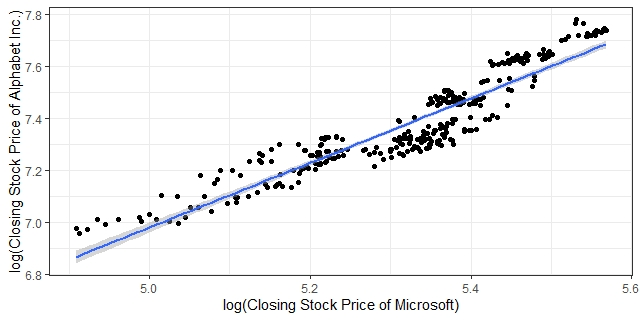
\includegraphics[width = .8\textwidth]{figures/plot6.jpeg}
    \caption{Scatterplot of Microsoft (MSFT) stock price vs Alphabet Inc (GOOGL) stock price}
    \label{fig:GvsM}
\end{figure}


\noindent Therefore we can see that there is a circular relationship between $SP_{G}$ and $SP_{M}$. From this and earlier considerations, we start with the following two structural equations,

\begin{align}
    SP_{G} & =\alpha_{0}+\alpha_{1}SP_{M}+\alpha_{2}C_{new}+\alpha_{3}PR_{Z}+\alpha_{4}PR_{S}+\alpha_{5}PR_{G}+\epsilon_{1} \label{eqn:structural-1} \\
    SP_{M} & =\beta_{0}+\beta_{1}SP_{G}+\beta_{2}C_{new}+\beta_{3}PR_{Z}+\beta_{4}PR_{S}+\beta_{5}PR_{M}+\epsilon_{2} \label{eqn:structural-2}
\end{align}

\noindent where $\epsilon_{1}$ and $\epsilon_{2}$ are zero-mean errors. These two equations represent a system of simultaneous equation, having $12$ structural parameters, namely $\alpha_{0}, \alpha_{1}, \alpha_{2}, \alpha_{3}, \alpha_{4}, \alpha_{5}, \beta_{0}, \beta_{1}, \beta_{2}, \beta_{3}, \beta_{4}$ and $\beta_{5}$. We shall obtain reduced form equations from here. Substituting the value of $SP_M$ from Eq.~\eqref{eqn:structural-2} in Eq.~\eqref{eqn:structural-1}, we obtain
%
\begin{align*}
    SP_{G} = & \left[\alpha_{0}+\alpha_{1}\beta_{0}\right]+\left[\alpha_{1}\beta_{1}\right]SP_{G}+\left[\alpha_{2}+\alpha_{1}\beta_{2}\right]C_{new}+\left[\alpha_{3}+\alpha_{1}\beta_{3}\right]PR_{Z}+\\
    & \left[\alpha_{4}+\alpha_{1}\beta_{4}\right]PR_{S}  +\alpha_{5}PR_{G}+\left[\alpha_{1}\beta_{5}\right]PR_{M}+\left[\epsilon_{1}+\alpha_{1}\epsilon_{2}\right]
\end{align*}

\noindent which yields,
%
\begin{align*}
    SP_{G} &  = \left[\dfrac{\alpha_{0}+\alpha_{1}\beta_{0}}{1-\alpha_{1}\beta_{1}}\right]+\left[\dfrac{\alpha_{1}\beta_{5}}{1-\alpha_{1}\beta_{1}}\right]PR_{M}+\left[\dfrac{\alpha_{2}+\alpha_{1}\beta_{2}}{1-\alpha_{1}\beta_{1}}\right]C_{new}+\\
    & \qquad \left[\dfrac{\alpha_{3}+\alpha_{1}\beta_{3}}{1-\alpha_{1}\beta_{1}}\right]PR_{Z}+\left[\dfrac{\alpha_{4}+\alpha_{1}\beta_{4}}{1-\alpha_{1}\beta_{1}}\right]PR_{S}  +\left[\dfrac{\alpha_{5}}{1-\alpha_{1}\beta_{1}}\right]PR_{G}+\left[\dfrac{\epsilon_{1}+\alpha_{1}\epsilon_{2}}{1-\alpha_{1}\beta_{1}}\right] \\
    & = G_{0}+G_{1}PR_{M}+G_{2}C_{new}+G_{3}PR_{Z}+G_{4}PR_{S}+G_{5}PR_{G}+\eta_{1}
\end{align*}

\noindent where $G_i$'s are the expressions that it is replacing (quantity inside the $(i+1)$-th bracket) for $0 \leq i \leq 5$ and $\eta_{1}$ is the error term inside the last parenthesis. Similarly, putting value of $SP_G$ from Eq.~\eqref{eqn:structural-1} into Eq.~\eqref{eqn:structural-2}, we obtain
%
\begin{align*}
    SP_{M} & =  \left[\dfrac{\beta_{0}+\beta_{1}\alpha_{0}}{1-\alpha_{1}\beta_{1}}\right]+\left[\dfrac{\beta_{1}\alpha_{5}}{1-\alpha_{1}\beta_{1}}\right]PR_{G}+\left[\dfrac{\beta_{2}+\beta_{1}\alpha_{2}}{1-\alpha_{1}\beta_{1}}\right]C_{new}+\\
    & \qquad  \left[\dfrac{\beta_{3}+\beta_{1}\alpha_{3}}{1-\alpha_{1}\beta_{1}}\right]PR_{Z}+ \left[\dfrac{\beta_{4}+\beta_{1}\alpha_{4}}{1-\alpha_{1}\beta_{1}}\right]PR_{S}  +\left[\dfrac{\beta_{5}}{1-\alpha_{1}\beta_{1}}\right]PR_{M}+\left[\dfrac{\epsilon_{2}+\beta_{1}\epsilon_{1}}{1-\alpha_{1}\beta_{1}}\right] \\
     & = M_{0}+M_{1}PR_{G}+M_{2}C_{new}+M_{3}PR_{Z}+M_{4}PR_{S}+M_{5}PR_{M}+\eta_{2}
\end{align*}

Combining these two derivations together, we obtain \textbf{two reduced form equations} as
%
\begin{align}
    SP_{G} = & G_{0}+G_{1}PR_{M}+G_{2}C_{new}+G_{3}PR_{Z}+G_{4}PR_{S}+G_{5}PR_{G}+\eta_{1} \label{eqn:reduced-1}\\
    SP_{M} = & M_{0}+M_{1}PR_{G}+M_{2}C_{new}+M_{3}PR_{Z}+M_{4}PR_{S}+M_{5}PR_{M}+\eta_{2} \label{eqn:reduced-2}
\end{align}

\noindent which now incorporates $12$ reduced form parameters. Since there are $12$ structural parameters and $12$ reduced form parameters, the simultaneous equation system is \textit{exactly identified} and we can get back the estimates of structural parameters from the estimates of reduced form parameters. 

Towards this, we first express the reduced form parameters in terms of structural parameters

\begin{center}
    \begin{minipage}{0.49\linewidth}
    \begin{align*}
 G_{0} &= \dfrac{\alpha_{0}+\alpha_{1}\beta_{0}}{1-\alpha_{1}\beta_{1}} \label{A1}\tag{A1}    \\
 G_{1} &= \dfrac{\alpha_{1}\beta_{5}}{1-\alpha_{1}\beta_{1}}    \label{A2}\tag{A2} \\
 G_{2} &= \dfrac{\alpha_{2}+\alpha_{1}\beta_{2}}{1-\alpha_{1}\beta_{1}}    \label{A3}\tag{A3} \\
 G_{3} &= \dfrac{\alpha_{3}+\alpha_{1}\beta_{3}}{1-\alpha_{1}\beta_{1}}    \label{A4}\tag{A4} \\
 G_{4} &= \dfrac{\alpha_{4}+\alpha_{1}\beta_{4}}{1-\alpha_{1}\beta_{1}}    \label{A5}\tag{A5} \\
 G_{5} &= \dfrac{\alpha_{5}}{1-\alpha_{1}\beta_{1}}    \label{A6}\tag{A6} \\
 \end{align*}
\end{minipage}
\begin{minipage}{0.49\linewidth}
    \begin{align*}
 M_{0} &= \dfrac{\beta_{0}+\beta_{1}\alpha_{0}}{1-\alpha_{1}\beta_{1}} \label{B1}\tag{B1}    \\
 M_{1} &= \dfrac{\beta_{1}\alpha_{5}}{1-\alpha_{1}\beta_{1}}      \label{B2}\tag{B2} \\
 M_{2} &= \dfrac{\beta_{2}+\beta_{1}\alpha_{2}}{1-\alpha_{1}\beta_{1}}   \label{B3}\tag{B3} \\
 M_{3} &= \dfrac{\beta_{3}+\beta_{1}\alpha_{3}}{1-\alpha_{1}\beta_{1}}   \label{B4}\tag{B4} \\
 M_{4} &= \dfrac{\beta_{4}+\beta_{1}\alpha_{4}}{1-\alpha_{1}\beta_{1}}   \label{B5}\tag{B5} \\
 M_{5} &= \dfrac{\beta_{5}}{1-\alpha_{1}\beta_{1}}    \label{B6}\tag{B6} \\
 \end{align*}
\end{minipage}
\end{center}

\noindent Now, from Eq.~\eqref{A2} and Eq.~\eqref{B6}, we obtain $\alpha_{1}=\dfrac{G_{1}}{M_{5}}$. Similarly, from Eq.~\eqref{B2} and Eq.~\eqref{A6}, we obtain $\beta_{1}=\dfrac{M_{1}}{G_{5}}$. Putting the expression of $\alpha_{1}$ in Eq.~\eqref{A2}, we get $\beta_{5}=(1-\alpha_{1}\beta_{1})M_{5}=M_{5}-\beta_{1}G_{1}$. In the same way, we obtain $\alpha_{5}=(1-\alpha_{1}\beta_{1})G_{5}=G_{5}-\alpha_{1}M_{1}$ putting the expression of $\beta_{1}$ in Eq.~\eqref{B2}. Also, we note that Eq.~\eqref{A1} and Eq.~\eqref{B1} can be expressed as

$$
\alpha_{0}+\alpha_{1}\beta_{0}=c_{1} \quad \text{and} \quad  \beta_{0}+\beta_{1}\alpha_{0}=d_{1}
$$

\noindent where $c_{1}=(1-\alpha_{1}\beta_{1})G_{0}$ and $d_{1}=(1-\alpha_{1}\beta_{1})M_{0}$. Solving these, we get

$$\alpha_{0}=\dfrac{c_{1}-\alpha_{1}d_{1}}{1-\alpha_{1}\beta_{1}} \quad \text{and} \quad \beta_{0}=\dfrac{d_{1}-\beta_{1}c_{1}}{1-\alpha_{1}\beta_{1}}$$

\noindent After some algebraic manipulations, these lead to
$$\alpha_{0}=G_{0}-\alpha_{1}M_{0} \quad \text{and} \quad  \beta_{0}=M_{0}-\beta_{1}G_{0}$$

\noindent Similarly, we can obtain expressions of $(\alpha_{2},\beta_{2})$ using Eq.~\eqref{A3} and \eqref{B3}; expressions of $(\alpha_{3},\beta_{3})$ using Eq.~\eqref{A4} and \eqref{B4}; expressions of $(\alpha_{4},\beta_{4})$ using Eq.~\eqref{A5} and \eqref{B5}.

Combining everything, the structural parameters can be written in terms of the reduced form parameters using a set of $12$ equations,
%
\begin{equation}
    \begin{split}
    & \alpha_{1}=G_{1}/M_{5}, \hspace{2mm} \beta_{1}=M_{1}/G_{5}, \\
    & \alpha_{0}=G_{0}-\alpha_{1}M_{0}, \hspace{2mm}  \beta_{0}=M_{0}-\beta_{1}G_{0},\\
    & \alpha_{2}=G_{2}-\alpha_{1}M_{2}, \hspace{2mm}  \beta_{2}=M_{2}-\beta_{1}G_{2},\\
    & \alpha_{3}=G_{3}-\alpha_{1}M_{3}, \hspace{2mm}  \beta_{3}=M_{3}-\beta_{1}G_{3},\\
    & \alpha_{4}=G_{4}-\alpha_{1}M_{4}, \hspace{2mm}  \beta_{4}=M_{4}-\beta_{1}G_{4},\\
    & \alpha_{5}=G_{5}-\alpha_{1}M_{1}, \hspace{2mm}  \beta_{5}=M_{5}-\beta_{1}G_{1}.
    \end{split}
    \label{eqn:expressions}
\end{equation}

\noindent This whole exercise suggests that we can solve the simulteneous equation system in Eq.~\eqref{eqn:structural-1} and \eqref{eqn:structural-2} by performing the solving the linear regression problem in Eq.~\eqref{eqn:reduced-1} and \eqref{eqn:reduced-2} and estimating the reduced form parameters. Then, an application of the formulas shown in Eq.~\eqref{eqn:expressions} can be used to recovered the structural parameters. However, before proceeding with the simultaneous linear regression, we notice that the variables in concern are time series variables. In other words, the observed samples are $SP_{G,t}, SP_{M,t}$ where $t$ is the time index, hence the errors are actually $\eta_{1t}, \eta_{2t}$ (The time index has been dropped in Eq.~\eqref{eqn:reduced-1} and Eq.~\eqref{eqn:reduced-2}). Therefore, a temporal dependence is expected to be present within each variable and the samples may be correlated, i.e. $\eta_{1t}$ and $\eta_{1(t-1)}$ may be correlated. Assuming that the errors are stationary, we consider an autoregressive model of order $1$ with $\eta_{it} = \phi_i \eta_{i(t-1)} + w_{it}$ for $i = 1, 2$, where $w_{it}$ is a white noise process with mean $0$ and variance $\sigma_{w,i}^2$. In this case,
%
$$
\text{Cov}(\eta_{it}, \eta_{i(t-s)}) = \phi_i^s\sigma^2_{w, i}/(1 - \phi_i^2), \qquad \text{ for } i = 1, 2
$$
%
\noindent where $\phi_i, \sigma_{w,i}^2$ are estimable parameters. Clearly, an ordinary least squares procedure would be inadequate for this, and hence a generalized least squares procedure can be used to estimate these parameters~\cite{fox2002time}. In particular, if we consider $\Sigma_i$ as the variance covariance matrix of $(\eta_{i1}, \eta_{i2}, \dots)$, then pre-multiplying each variable in Eq.~\eqref{eqn:reduced-1} and \eqref{eqn:reduced-2} by $\Sigma_i^{-1/2}$ turns the system into usual linear regression model with independent samples.

However, inclusion of number of covid cases as an explanatory variable also creates another problem. Many scientists have warned time and again that covid cases and deaths are being undercounted throughout the world~\cite{covid-underreporting}. Countries like France, Italy, the United States of America, Iran and Spain have extremely high numbers of undetected and underreported cases~\cite{Lau-2020}. Thus, the variable $C_{new}$ involves measurement error and hence is correlated with the error terms $\eta_{1t}, \eta_{2t}$. This induces an endogeneity problem. Consequently, the parameters present in the two reduced form equations \eqref{eqn:reduced-1} and \eqref{eqn:reduced-2} can not be estimated unbiasedly and consistently. To overcome this problem, we introduce an instrumental variable namely covid search, denoted by $C_{s}$. This is a similar normalized popularity rating of the search term ``covid" or related topics which is collected from Google trends dataset along with other search terms. Since square root transformation was applied to form $C_{new}$, $C_s$ also denotes the square root transformation of the normalized popularity rating. We find that this has a correlation $0.9605317$ with $C_{new}$. On the other hand, intuitively $C_{s}$ should not be directly related with the two stock prices. Therefore, it can be used as an instrumental variable to estimate the parameters in Eq.~\eqref{eqn:reduced-1} and \eqref{eqn:reduced-2}. Using $C_s$ as the instrumental variable, we may use IV regression method to estimate these reduced form parameters.

Although the problem of endogeneity through measurement error in number of covid cases worldwide is suspected, one may use Hausman test of endogeneity to confirm the suspicion. Let $\widehat{G}_{IV}$ and $\widehat{G}_{OLS}$ be the IV and the OLS estimates obtained. Note that after transforming the data into independendent samples through pre-multiplying estimated $\widehat{\Sigma}_i$, the obtained OLS estimate $\widehat{G}_{OLS}$ is actually a GLS estimate. To test the endogeneity hypothesis 
\begin{align*}
    & H_{0G}: C_{new} \text{ is not endogeneous in Eq. } \eqref{eqn:reduced-1}\\
    & H_{1G}: C_{new} \text{ is endogeneous in Eq. }\eqref{eqn:reduced-2}
\end{align*}

\noindent we can use the Hausman test statistic 
%
$$n \left(\widehat{G}_{IV}-\widehat{G}_{OLS}\right)^{\intercal}\left(\mathbb{V}\text{ar}(\widehat{G}_{IV})-\mathbb{V}\text{ar}(\widehat{G}_{OLS})\right)^{-1}\left(\widehat{G}_{IV}-\widehat{G}_{OLS}\right)$$

\noindent which under the null hypothesis $H_{0G}$, follows a chi-squared distribution $\chi_p^2$ with degrees of freedom $p$ equal to the number of parameters. In our case, $p = 6$. We shall reject the null hypothesis and conclude that there is an endogeneity problem if the value of the observed statistic exceeds the critical value obtained from the $100(1-\alpha)$-th quantile of $\chi_6^2$ distribution at $\alpha$ level of significance. In a very similar manner, test for the presence of endogeneity in Eq.~\eqref{eqn:reduced-2} can also be performed.

\section{Results and Discussions}

Applying GLS along with IV estimation technique for estimate the parameters, we obtain
\begin{align*}
    \widehat{G}_{OLS} & = \left(7.30212, -3.67621\times 10^{-4}, 1.22134\times 10^{-4}, 8.74257\times 10^{-4}, -8.40212\times 10^{-4},\right.\\
    & \qquad \qquad \left. -11.65843\times10^{-4} \right) \text{ and; }\\
    \widehat{G}_{IV} & = \left(7.29918, -3.82965\times 10^{-4}, 1.34618\times 10^{-4}, -8.49866\times 10^{-4},\right.\\
    & \qquad \qquad \left. -8.19565\times 10^{-4}, 11.45836\times 10^{-4}\right)
\end{align*}

\noindent We observe that in $\widehat{G}_{IV}$ coefficient of google meet search is positive. This tells that the stock price of Alphabet Inc increases as google meet search increases. It is also noted that the estimated coefficient of zoom search is negative in $\widehat{G}_{IV}$. This can be interpreted as evidence in favour of the fact that increased popularity of rival video conferencing service results into decrease in stock price. The signs of coefficients estimated using OLS are difficult to interpret. The value of the Hausman test statistic is $40.60228$ with a p-value $=3.467842\times 10^{-7}$. Hence, we reject the null hypothesis that $C_{new}$ is not endogenous at $0.01$ level of significance. This confirms our earlier assertion that $C_{new}$ is endogeneous in the regression equation \eqref{eqn:reduced-1}. Finally, it yields a multiple R-squared value equal to $0.869$, which suggests a very good fit of the linear regression. 

Similarly, for the linear regression given in Eq.~\eqref{eqn:reduced-2}, the estimates turned out to be 
\begin{align*}
    \widehat{M}_{OLS} & = \left(5.22482, -8.58101\times 10^{-5}, 1.68968\times 10^{-4}, 4.05142\times 10^{-4}, -8.77877\times 10^{-4}, \right.\\
    & \qquad \qquad \left. -1.91413\times 10^{-4} \right) \text{ and; }\\
    \widehat{M}_{IV} & = \left(5.2204,  -5.56586\times 10^{-5}, 1.87783\times 10^{-4}, -3.68382\times 10^{-4}, -8.46759\times 10^{-4},\right.\\
    & \qquad \qquad \left. 2.14539\times 10^{-4} \right)
\end{align*}
The signs of coefficients in $\widehat{M}_{IV}$ are similar to those of $\widehat{G}_{IV}$. For example, the estimated coefficient of zoom search is negative in $\widehat{M}_{IV}$ too. We also observe that in $\widehat{M}_{IV}$, coefficient of microsoft teams search is positive. This can be interpreted as evidence in favour of the fact that increased popularity of microsoft teams generally results into increased stock price of Microsoft corporation. Again, the signs of components of $\widehat{M}_{OLS}$ are difficult to interpret in this manner. The observed value of the Hausman test statistic turns out to be $99.17337$ with a p-value $3.732403\times 10^{-19}$. Therefore, we reject the null hypothesis that $C_{new}$ is not endogeneous again at $0.01$ level of significance and confirm that the data shows sufficient evidence to suspect that $C_{new}$ is endogeneous in the linear regression equation~\eqref{eqn:reduced-2} as well. Finally, it yields a multiple R-squared value equal to $0.742$, which suggests a very good fit of the linear regression considered here. 

We have seen in Section~\ref{sec:methods} how we can get back the estimates of structural parameters from the estimates of the reduced form parameters. Using the relationships derived there, we obtain the estimates of $\alpha=(\alpha_{0}, \alpha_{1}, \alpha_{2}, \alpha_{3}, \alpha_{4}, \alpha_{5})$ and $\beta=(\beta_{0}, \beta_{1}, \beta_{2}, \beta_{3}, \beta_{4}$, $\beta_{5})$ from $\widehat{G}_{IV}$ and $\widehat{M}_{IV}$. The resulting estimates, if put back into Eq.~\eqref{eqn:structural-1} and \eqref{eqn:structural-2} yields the simultaneous regression equations as 
\begin{equation}
    SP_{G} = 16.6178-1.785SP_{M}+0.00047C_{new}-0.0015PR_{Z}-0.0023PR_{S}+0.00105PR_{G} \label{eqn:structural-1-solved}
\end{equation}
\noindent and
\begin{multline}
SP_{M} = 5.57495-0.0485SP_{G}+0.000194C_{new}-0.00041PR_{Z}-0.00089PR_{S}\\+0.000195PR_{M} \label{eqn:structural-2-solved}    
\end{multline}

\begin{figure}[ht]
    \centering
    \begin{subfigure}{0.47\textwidth}
       \centering
       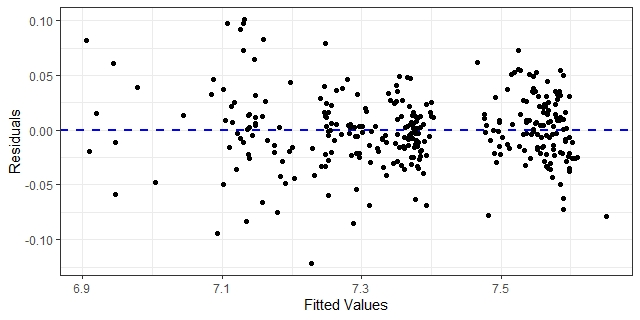
\includegraphics[width = \textwidth]{figures/plot7.jpeg}
       \caption{Fitted values vs Corrected Residuals for Regression Eq.~\eqref{eqn:reduced-1}}
       \label{fig:residuals-google}
    \end{subfigure}
    \hfill
    \begin{subfigure}{0.47\textwidth}
       \centering
       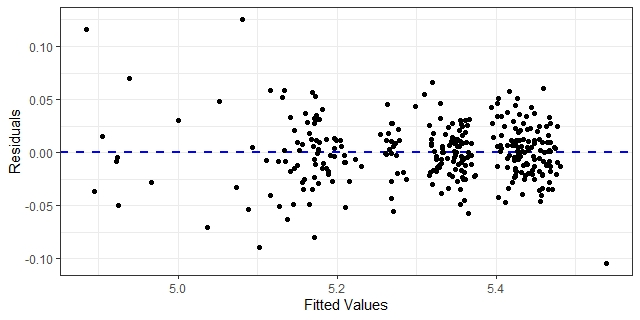
\includegraphics[width = \textwidth]{figures/plot8.jpeg}
       \caption{Fitted values vs Corrected Residuals for Regression Eq.~\eqref{eqn:reduced-2}}
       \label{fig:residuals-microsoft}
    \end{subfigure}
    \begin{subfigure}{0.47\textwidth}
       \centering
       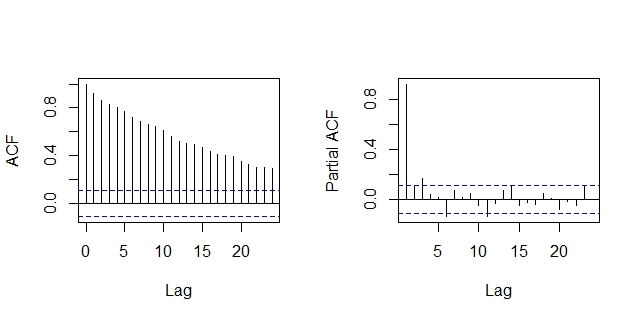
\includegraphics[width = \textwidth]{figures/plot7a.jpeg}
       \caption{ACF and PACF plots of the difference between true stock price of Google and Prediction from linear regression model}
       \label{fig:acf-google}
    \end{subfigure}
    \hfill
    \begin{subfigure}{0.47\textwidth}
       \centering
       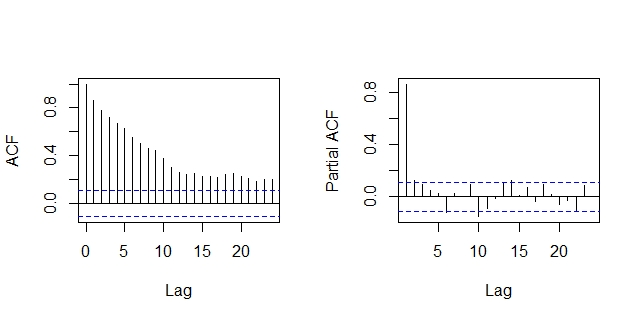
\includegraphics[width = \textwidth]{figures/plot8a.jpeg}
       \caption{ACF and PACF plots of the difference between true stock price of Microsoft and Prediction from linear regression model}
       \label{fig:acf-microsoft}
    \end{subfigure}
    \caption{Residual Diagnostics}
\end{figure}

Finally, to test whether the assumptions of linearity and autoregressive residuals were correct, we can simply plot the corrected residuals and the fitted values from the transformed regression models with independent samples (The one obtained by pre-multiplying with $\Sigma_i^{-1/2}$). As shown in Figures~\ref{fig:residuals-google} and \ref{fig:residuals-microsoft}, both of the residual plots show a random distribution of residuals to both sides of the x-axis. Since no visible pattern is found in the residuals, it seems the linear regression model was an adequate choice. Also, Figures~\ref{fig:acf-google} and \ref{fig:acf-microsoft} plots the ACF and PACF plots of the errors in prediction of the final stock prices, i.e. the difference between the true stock prices and the prediction from the two linear regression models (exponential of the fitted values from Eq.~\eqref{eqn:reduced-1} and \eqref{eqn:reduced-2}). These plots support our assumption that $\eta_{it}$'s have an autoregressive model of order $1$, as indicated in Section~\ref{sec:methods}.



\section{Conclusion}

From the simultaneous equations obtained in Eq.~\eqref{eqn:structural-1-solved} and Eq.~\eqref{eqn:structural-2-solved}, we observe the following;


\begin{enumerate}
    \item Google and Microsoft stock price are contrasting in nature. Each one has a decreasing effect on the other companies stock prices.
    \item In both equations, the number of new covid cases has positive coefficients. In other words, both companies' stock prices boomed during the covid19 outbreak. 
    \item Zoom and Skype search have a negative impact. Skype although owned by Microsoft is not boosted for sale during the covid period. 
    \item Google meet search has positive feedback for Alphabet Inc. stock price, and similar for Microsoft teams search and Microsoft Corporation.
\end{enumerate}

The results of our study also substantiate the claim that countries have grossly understated covid caseloads. Underreporting the caseload has far-reaching consequences for how a country responds. Governments could fail to direct funding and other resources to an area in need if the virus seems to have a relatively low threat there. Moreover, accurate counts provide scientists with crucial information about the virus. On the contrary, erroneously low tallies—due to a lack of testing or, in some cases, pressure or policies by government officials—can affect individual behavior~\cite{covid-underreporting}. If people feel there is a low risk of contracting COVID-19 in their community, they could choose to interact more with others, resulting in an increased caseload. 

Finally, in answer to the objective of this study, we find that there is a significant effect of covid on these two stock prices. Although most of the economy suffered heavily during the start of the pandemic, these two companies could produce their respective online learning and video conferencing tools meeting their demands, and in turn, earning a significant boost in their stock prices.



\bibliographystyle{plain}
\bibliography{references}
\nocite{*}


\end{document}









